\documentclass[11pt,a4paper]{article}
\usepackage{natbib}
\renewcommand{\bibname}{References}
%\usepackage[natbibapa]{apacite}
\usepackage{amsmath, amsthm, amssymb}\allowdisplaybreaks[3]
%\usepackage{marginnote}
\usepackage[dvips]{graphicx,color}
\usepackage{psfrag}
\usepackage[nottoc]{tocbibind}

% Define geometry
\setlength{\marginparwidth}{0mm}
\usepackage[width=15cm,height=24cm,includemp]{geometry}
\addtolength{\footskip}{10mm}

% No indentation for new paragraphs
\usepackage[parfill]{parskip}[2001/04/09]

% Define page style
\usepackage{fancyhdr}
\pagestyle{fancy}
\renewcommand{\headrulewidth}{0pt}
\lhead{}
\chead{}
\rhead{}
\renewcommand{\footrulewidth}{0.4pt}
\lfoot{\scriptsize{HGF Toolbox Manual}}
\cfoot{\thepage}
% File name and version in the footer
\rfoot{\scriptsize{\input{"|git rev-list --max-count=1 HEAD | cut -c 1-8"}}}

% Customize figure captions
\usepackage[footnotesize,normal,bf,up]{caption}
\renewcommand{\captionfont}{\footnotesize\itshape}

% Set frenchspacing
\frenchspacing

% Customize the 'enumerate' environment
\renewcommand{\labelenumi}{\arabic{enumi})}
\renewcommand{\labelenumii}{\alph{enumii})}
\renewcommand{\labelenumiii}{\roman{enumiii})}

% Do not number sections
\setcounter{secnumdepth}{3}

% Adjust equation numbering
\numberwithin{equation}{section}

% Create missing math symbols
\usepackage{amsfonts}
\newcommand{\N}{\ensuremath{\mathbb{N}}}
\newcommand{\Z}{\ensuremath{\mathbb{Z}}}
\newcommand{\Q}{\ensuremath{\mathbb{Q}}}
\newcommand{\R}{\ensuremath{\mathbb{R}}}
\newcommand{\C}{\ensuremath{\mathbb{C}}}
\newcommand{\Nc}{\ensuremath{\mathcal{N}}}
\newcommand{\Zc}{\ensuremath{\mathcal{Z}}}
\newcommand{\Lc}{\ensuremath{\mathcal{L}}}

\newcommand{\dd}{\:\mathrm{d}}
\newcommand{\dt}{\:\mathrm{d}t}
\newcommand{\dx}{\:\mathrm{d}x}

\newcommand{\me}{\mathrm{e}}

\newcommand{\argmin}{\operatornamewithlimits{argmin}}
\newcommand{\argmax}{\operatornamewithlimits{argmax}}

% Shortcuts
\newcommand{\mr}{\marginpar}
\newcommand{\mn}{\marginnote}
\newcommand{\rr}{\raggedright}
\newcommand{\fn}{\footnotesize}
\newcommand{\sz}{\scriptsize}
\newcommand{\dst}{\displaystyle}
\newcommand{\ol}{\overline}
\newcommand{\vth}{\vartheta}
\newcommand{\ve}{\varepsilon}
\newcommand{\la}{\lambda}
\newcommand{\sa}{\sigma}
\newcommand{\vph}{\varphi}
\newcommand{\ty}{\tilde{y}}
\newcommand{\ub}{\underbrace}
\newcommand{\sm}{\setminus}
\newcommand{\T}{\mathrm{T}}
\newcommand{\tr}{\mathrm{tr}}
\newcommand{\ra}{\rightarrow}
\newcommand{\td}[2]{\frac{\mathrm{d} #1}{\mathrm{d} #2}}
\newcommand{\tdd}[2]{\frac{\mathrm{d^2} #1}{\mathrm{d} {#2}^2}}
\newcommand{\pd}[2]{\frac{\partial #1}{\partial #2}}
\newcommand{\pdd}[2]{\frac{\partial^2 #1}{\partial {#2}^2}}
\newcommand{\fd}[2]{\frac{\delta #1}{\delta #2}}

\newcommand{\slmn}{\setlength{\lineskip}{0.5pt plus0.5pt minus0.5pt}}

\begin{document}

\section*{\huge HGF Toolbox Manual}
\label{manual}

\tableofcontents
\pagebreak

\section{Introduction}
\label{sec:intro}

The HGF toolbox provides generic methods for fitting time series
models using Bayesian inference.

It is built around the Hierarchical Gaussian Filter (HGF). It may
therefore not contain your favorite time series model. However, the
toolbox's modular nature should make it easy to add new models (see
Section \ref{sec:addmod} below).

The HGF was introduced in \citet{mathys_bayesian_2011} and elaborated
in \citet{mathys_uncertainty_2014}. Whenever you make use of one of
the various models based on the HGF, please cite these papers.

As shown in Figure \ref{Slide1}, the toolbox assumes a framework where
an agent in the broadest sense (e.g., a human being, an animal, a
machine, the stock market, etc.)  receives a time series of inputs to
which it reacts by emitting a time series of responses. In particular,
this process is modeled by the combination of a perceptual (sc. state
space) model and an observation (sc. decision or response) model. The
perceptual model is the time series model on which the agent bases its
responses; the response model describes how the agent makes decisions
based on its perceptual inference.

\begin{figure}[h]
\renewcommand{\baselinestretch}{1}
\begin{center}
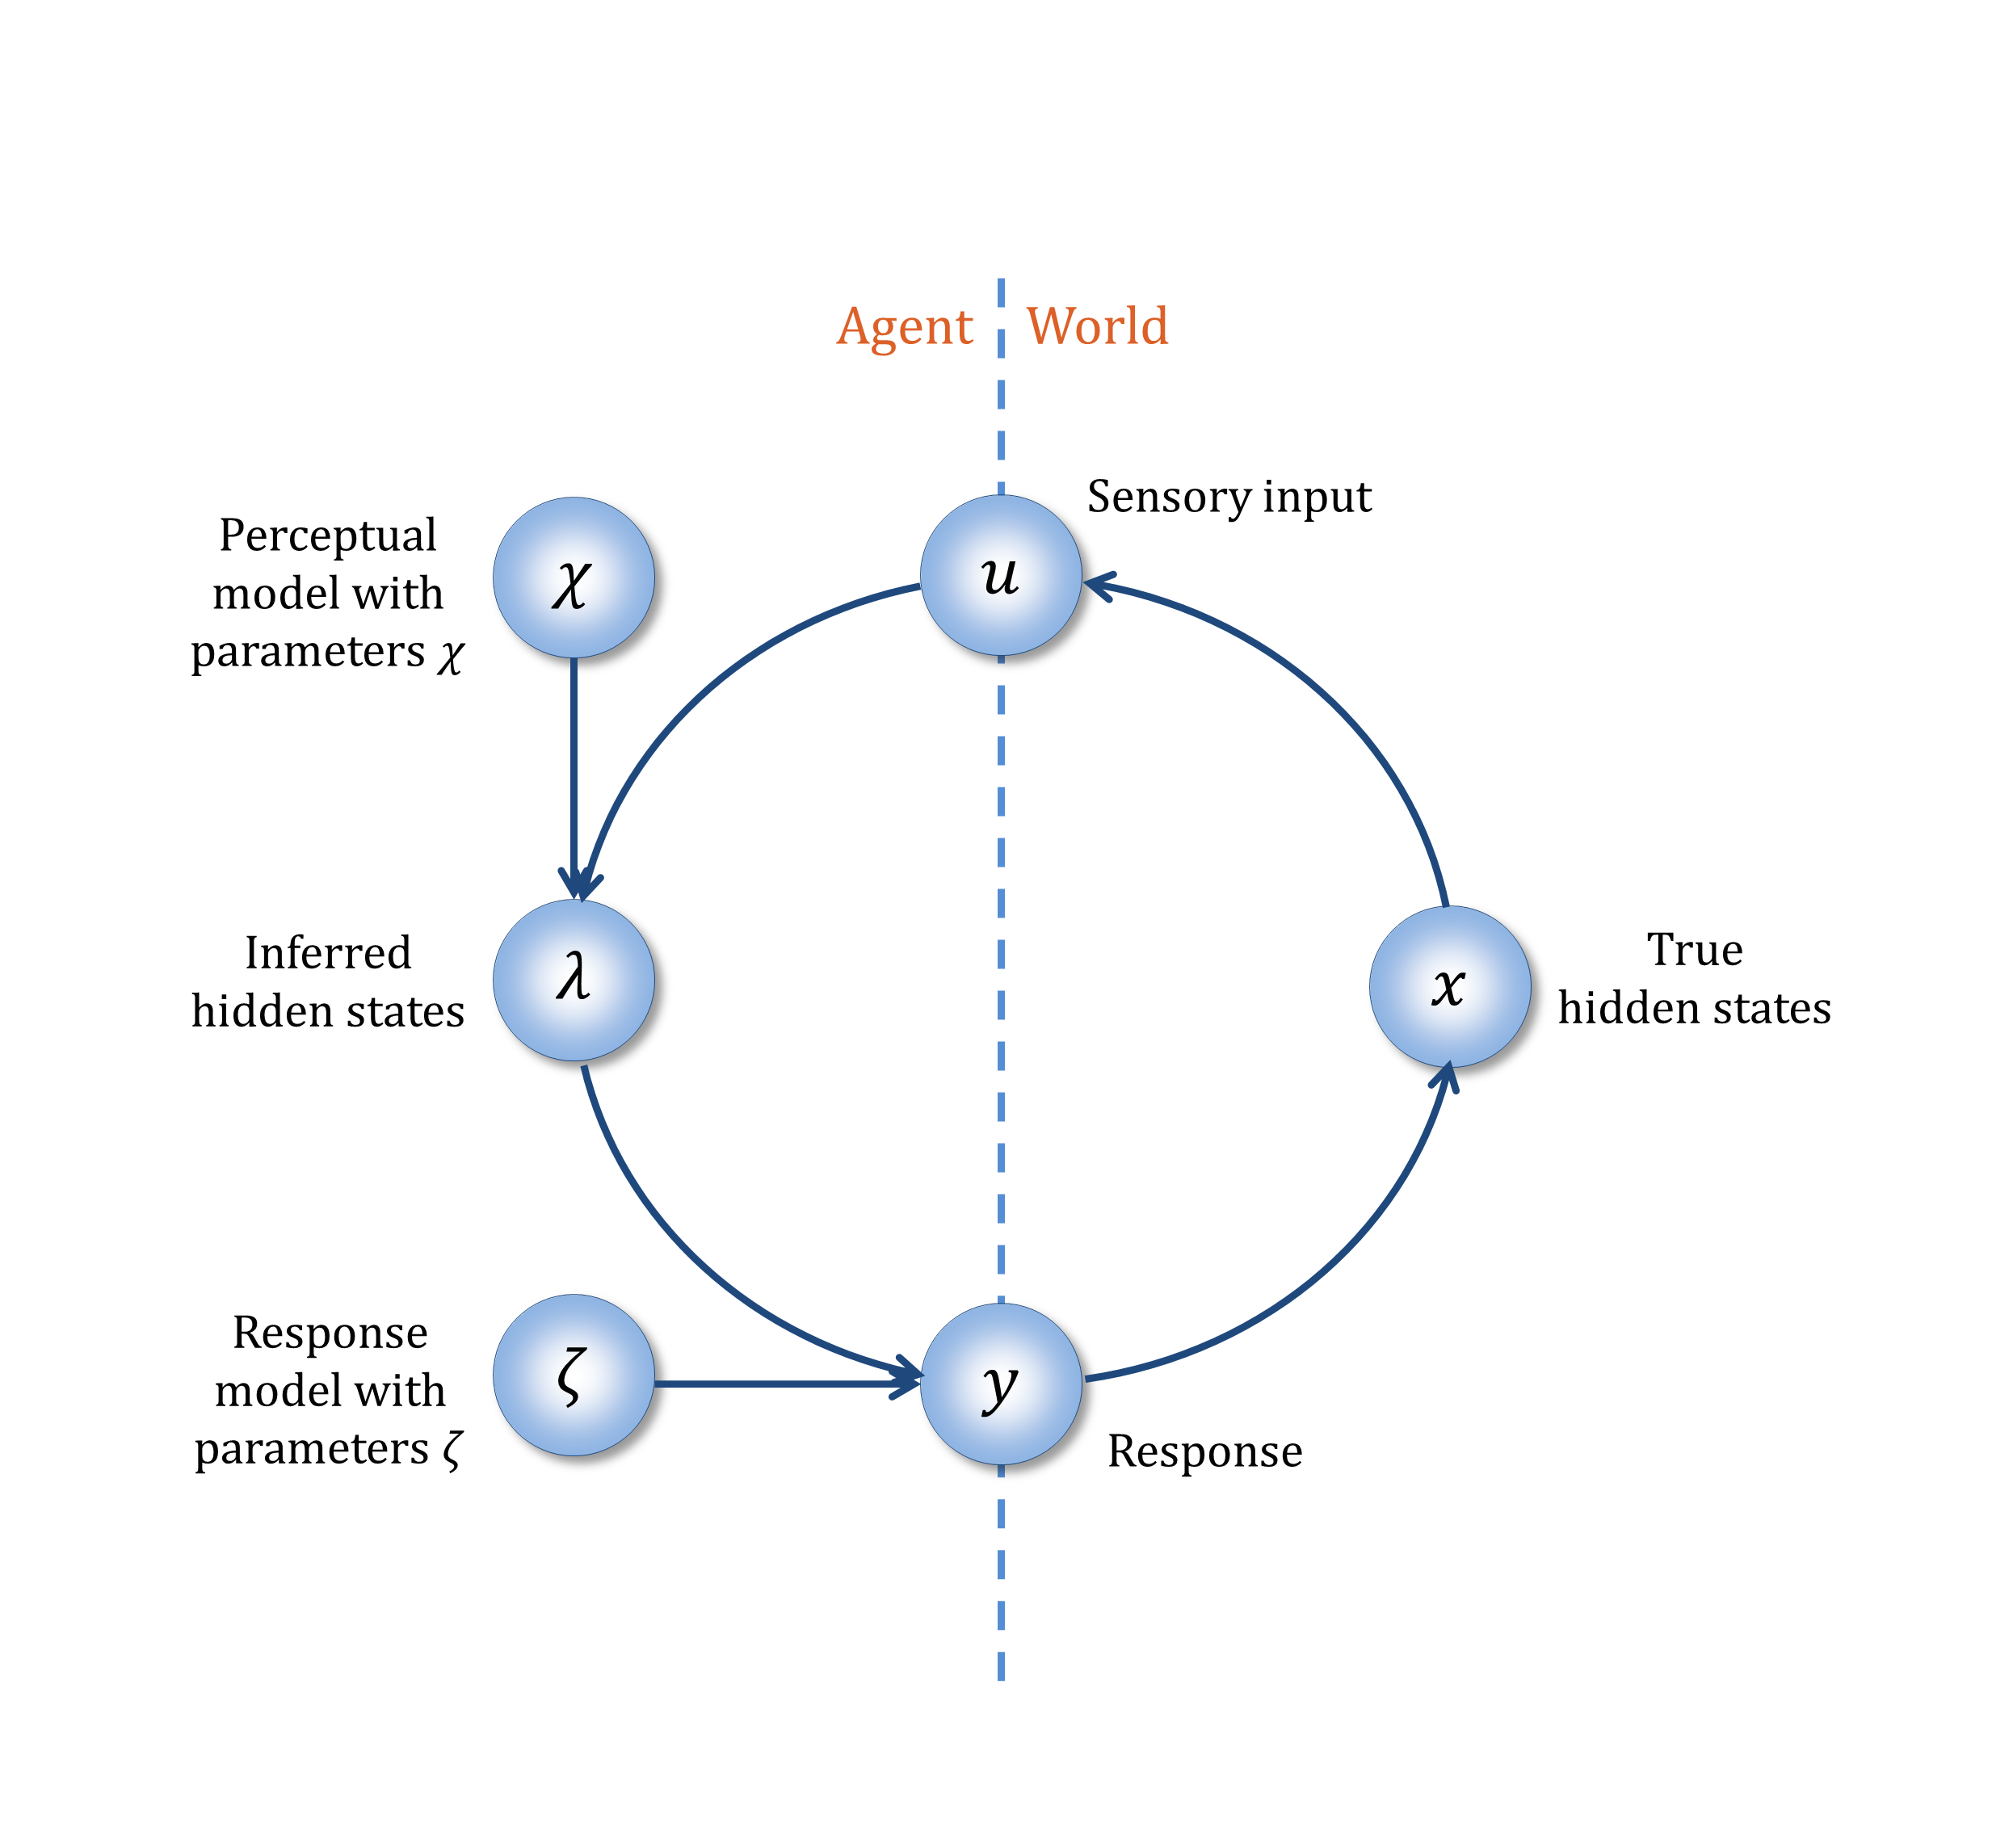
\includegraphics[width=14cm]{Graphics/Slide1}

\vspace{1ex}
\parbox{14cm}{\caption{\label{Slide1}
\textbf{\upshape General framework.}
An agent is connect to the external world by its sensory input $u$
and by the actions $y$ it takes in response. Inputs are used to infer
hidden states of the world, beliefs $\lambda$ about which are encoded
internally. Inference rests on a perceptual model parameterized by
$\chi$. Actions depend on beliefs $\lambda$ and are described by a
response model parameterized by $\zeta$.}}
\end{center}
\end{figure}
 
Note that what we refer to here as the observation model describes a
"second-order" observation in the sense that the perceptual model
already contains a ("first-order") observation part that describes how
perceptual states relate to inputs. This implements the "observing the
observer" framework described in \citet{daunizeau_observing_2010}.


\section{Usage}
\label{sec:usage}

There are two main ways to use the HGF toolbox. The first is to fit
various combinations of perceptual and observation models to observed
responses (Figure \ref{Slide2}).

\begin{figure}[h]
\renewcommand{\baselinestretch}{1}
\begin{center}
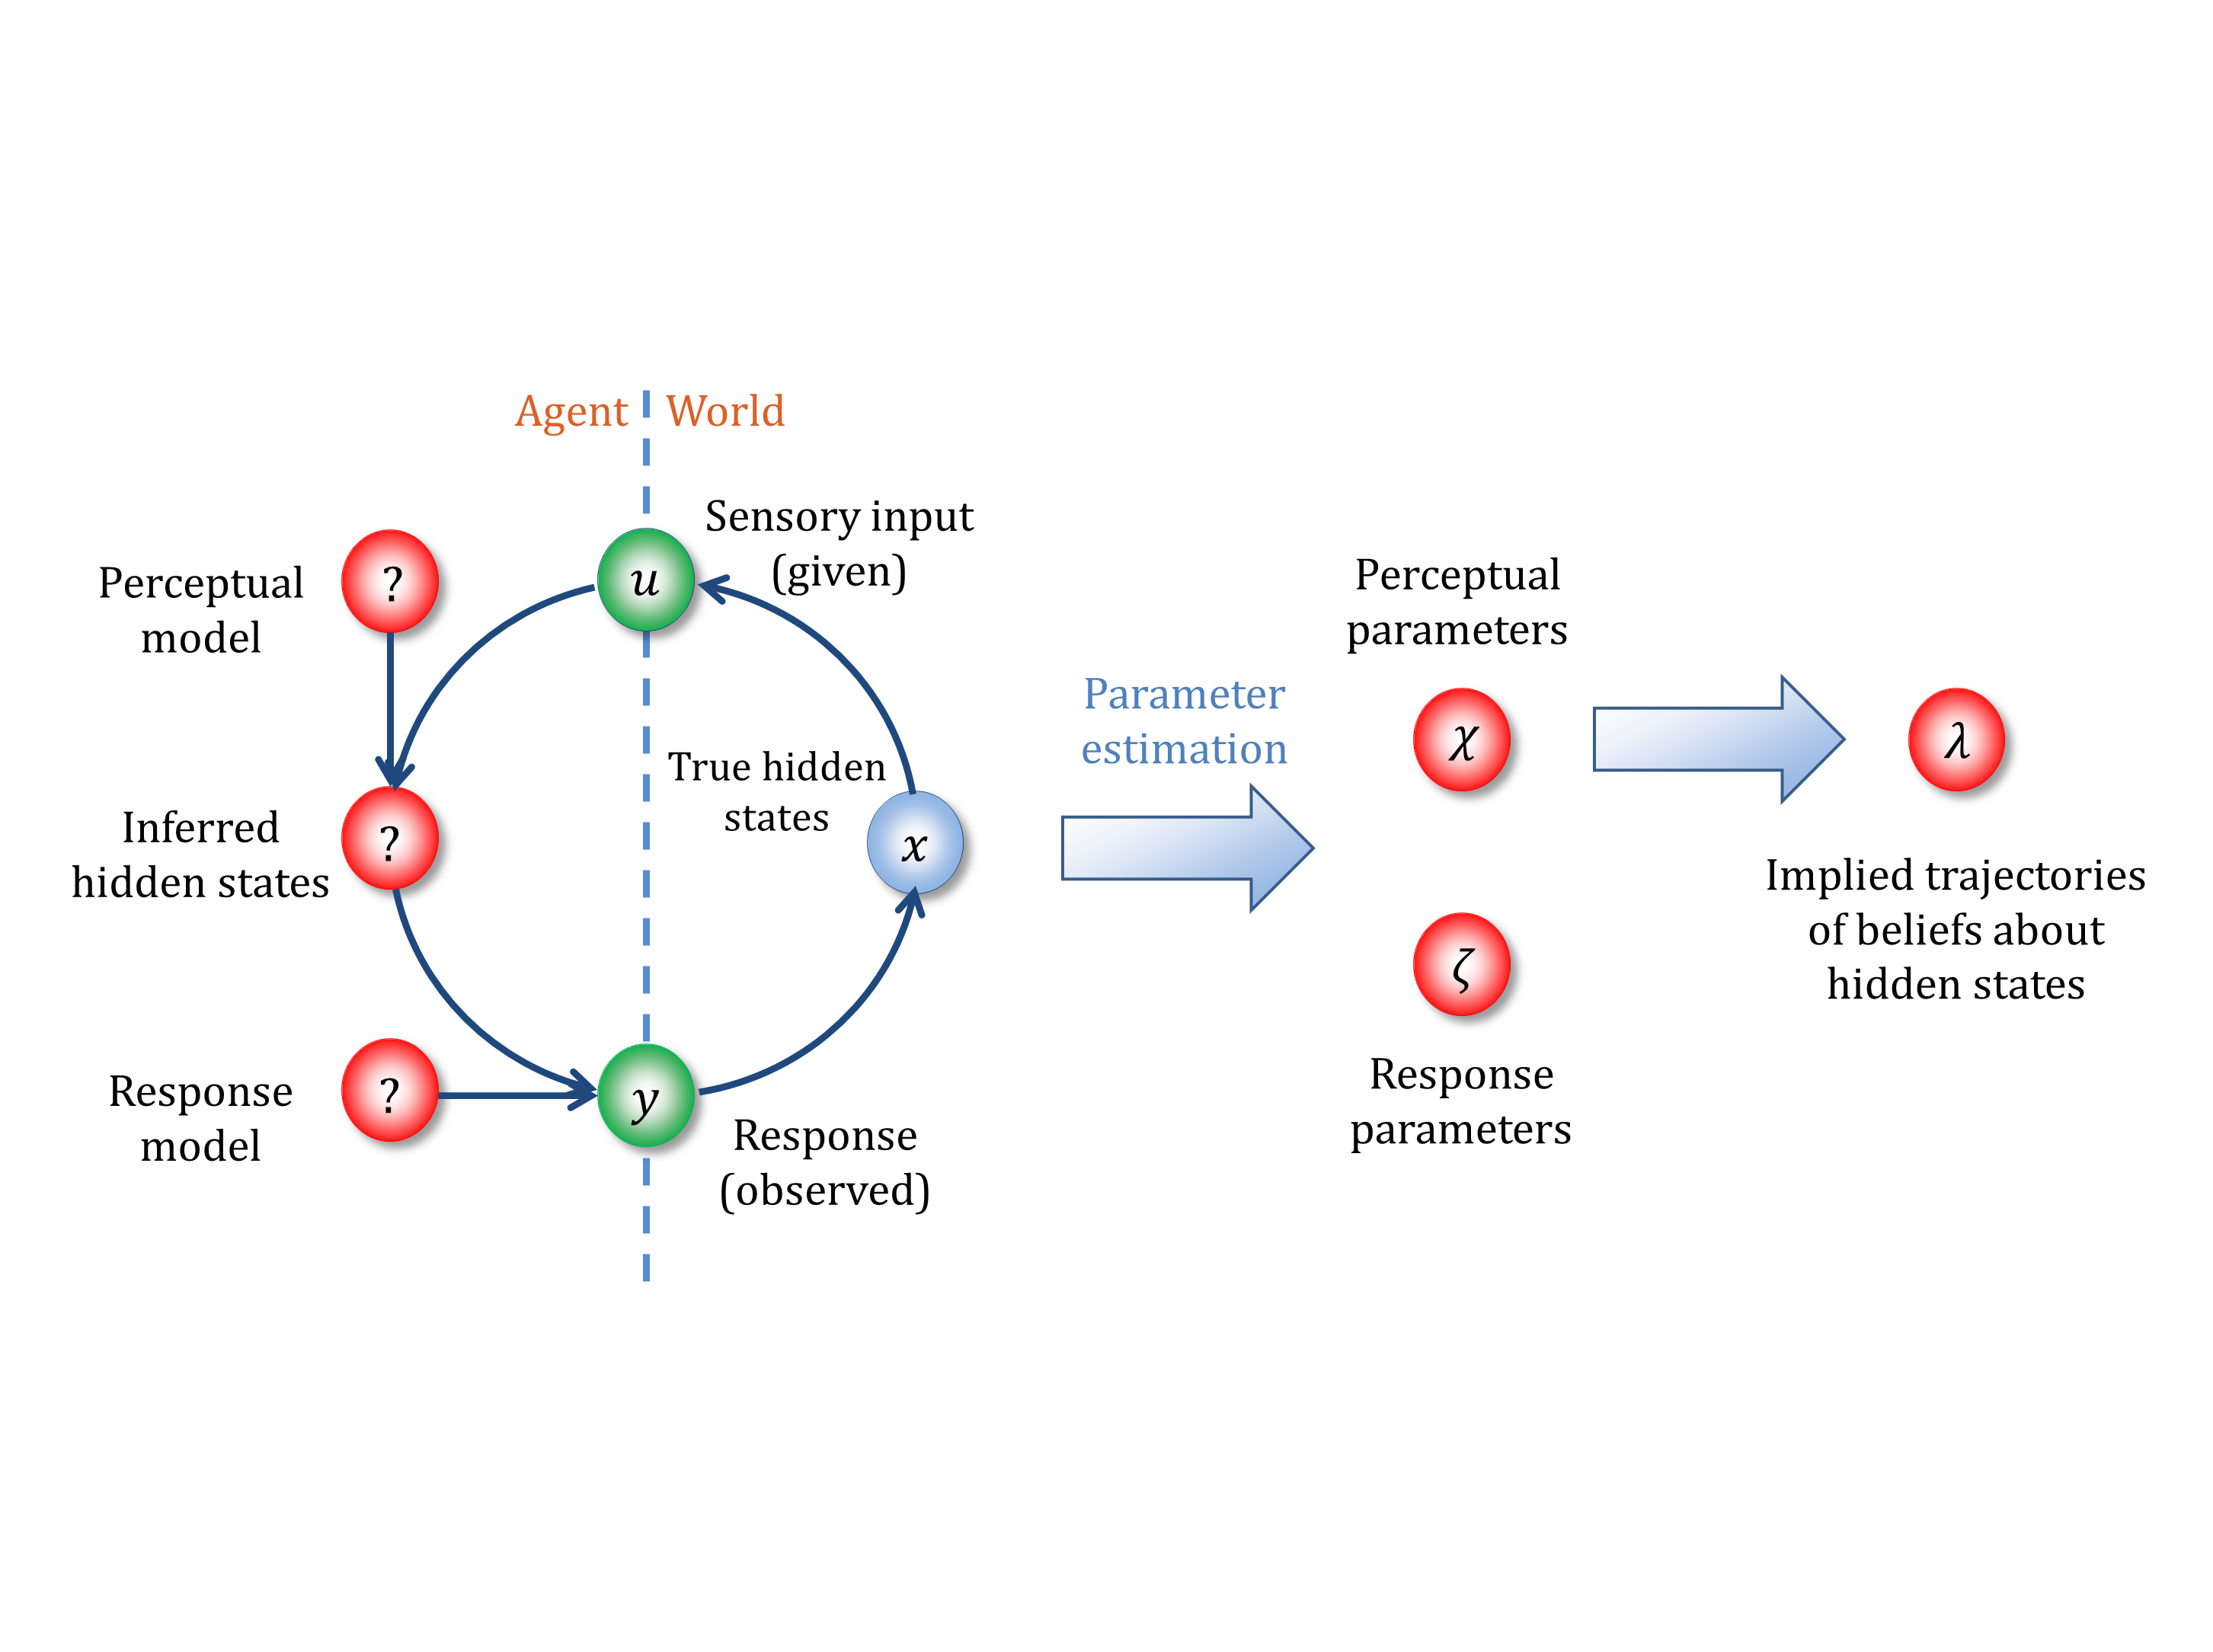
\includegraphics[width=14cm]{Graphics/Slide2}

\vspace{1ex}
\parbox{14cm}{\caption{\label{Slide2}
\textbf{\upshape Parameter estimation.}
When both inputs and responses are known, the parameters of the
perceptual and the response model can be estimated, and the resulting
estimate of the perceptual parameters implies trajectories of beliefs
about hidden external states. Parameter estimation is performed by the
function \texttt{\upshape tapas\_fitModel(...)}.}}
\end{center}
\end{figure}
 
The second main usage is to simulate the trajectories of beliefs about
external states, and responses based on these beliefs (Figure
\ref{Slide3}).

\begin{figure}[h]
\renewcommand{\baselinestretch}{1}
\begin{center}
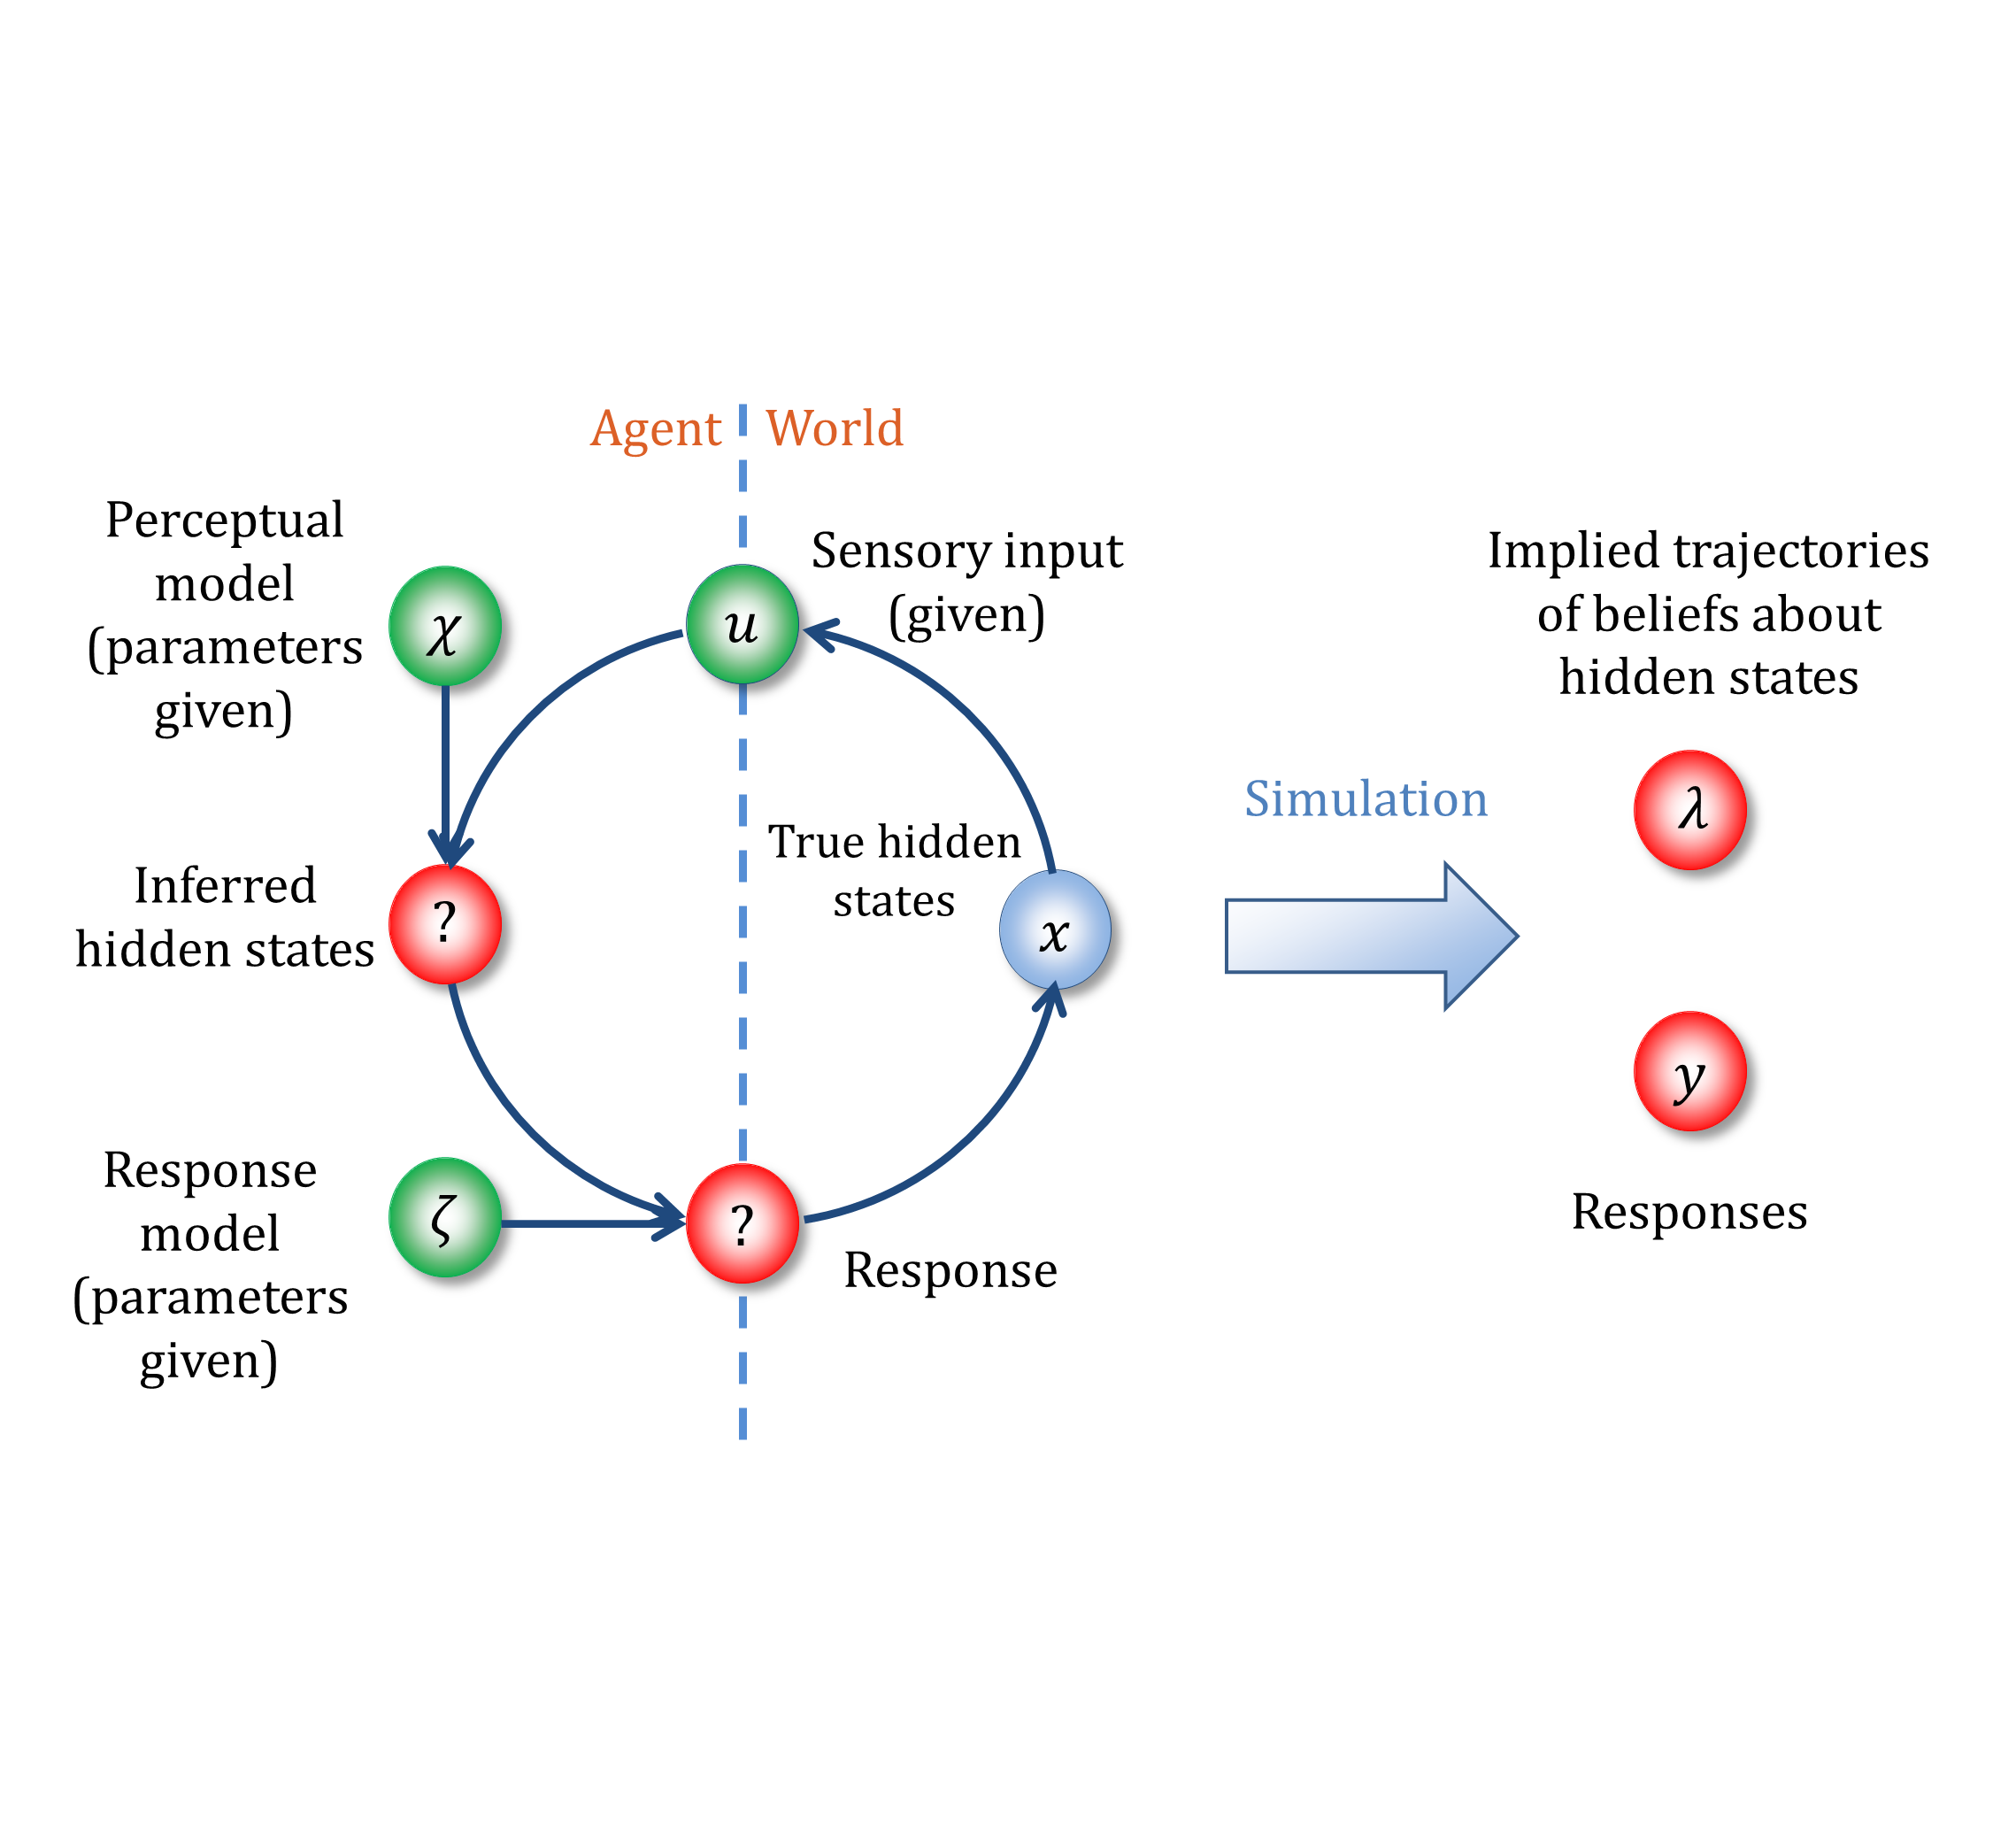
\includegraphics[width=14cm]{Graphics/Slide3}

\vspace{1ex}
\parbox{14cm}{\caption{\label{Slide3}
\textbf{\upshape Simulation of belief trajectories and responses.}
When the parameters of the perceptual and the response model are given
in addition to the inputs, belief trajectories and responses can be
simulated. This is performed by the function \texttt{\upshape
  tapas\_simModel(...)}.}}
\end{center}
\end{figure}
 
In simpler cases (e.g., when simply filtering inputs), only the
evolution of the perceptual inference is of interest and the the
specification of a response model is unnecessary (Figure
\ref{Slide4}).

\begin{figure}[h]
\renewcommand{\baselinestretch}{1}
\begin{center}
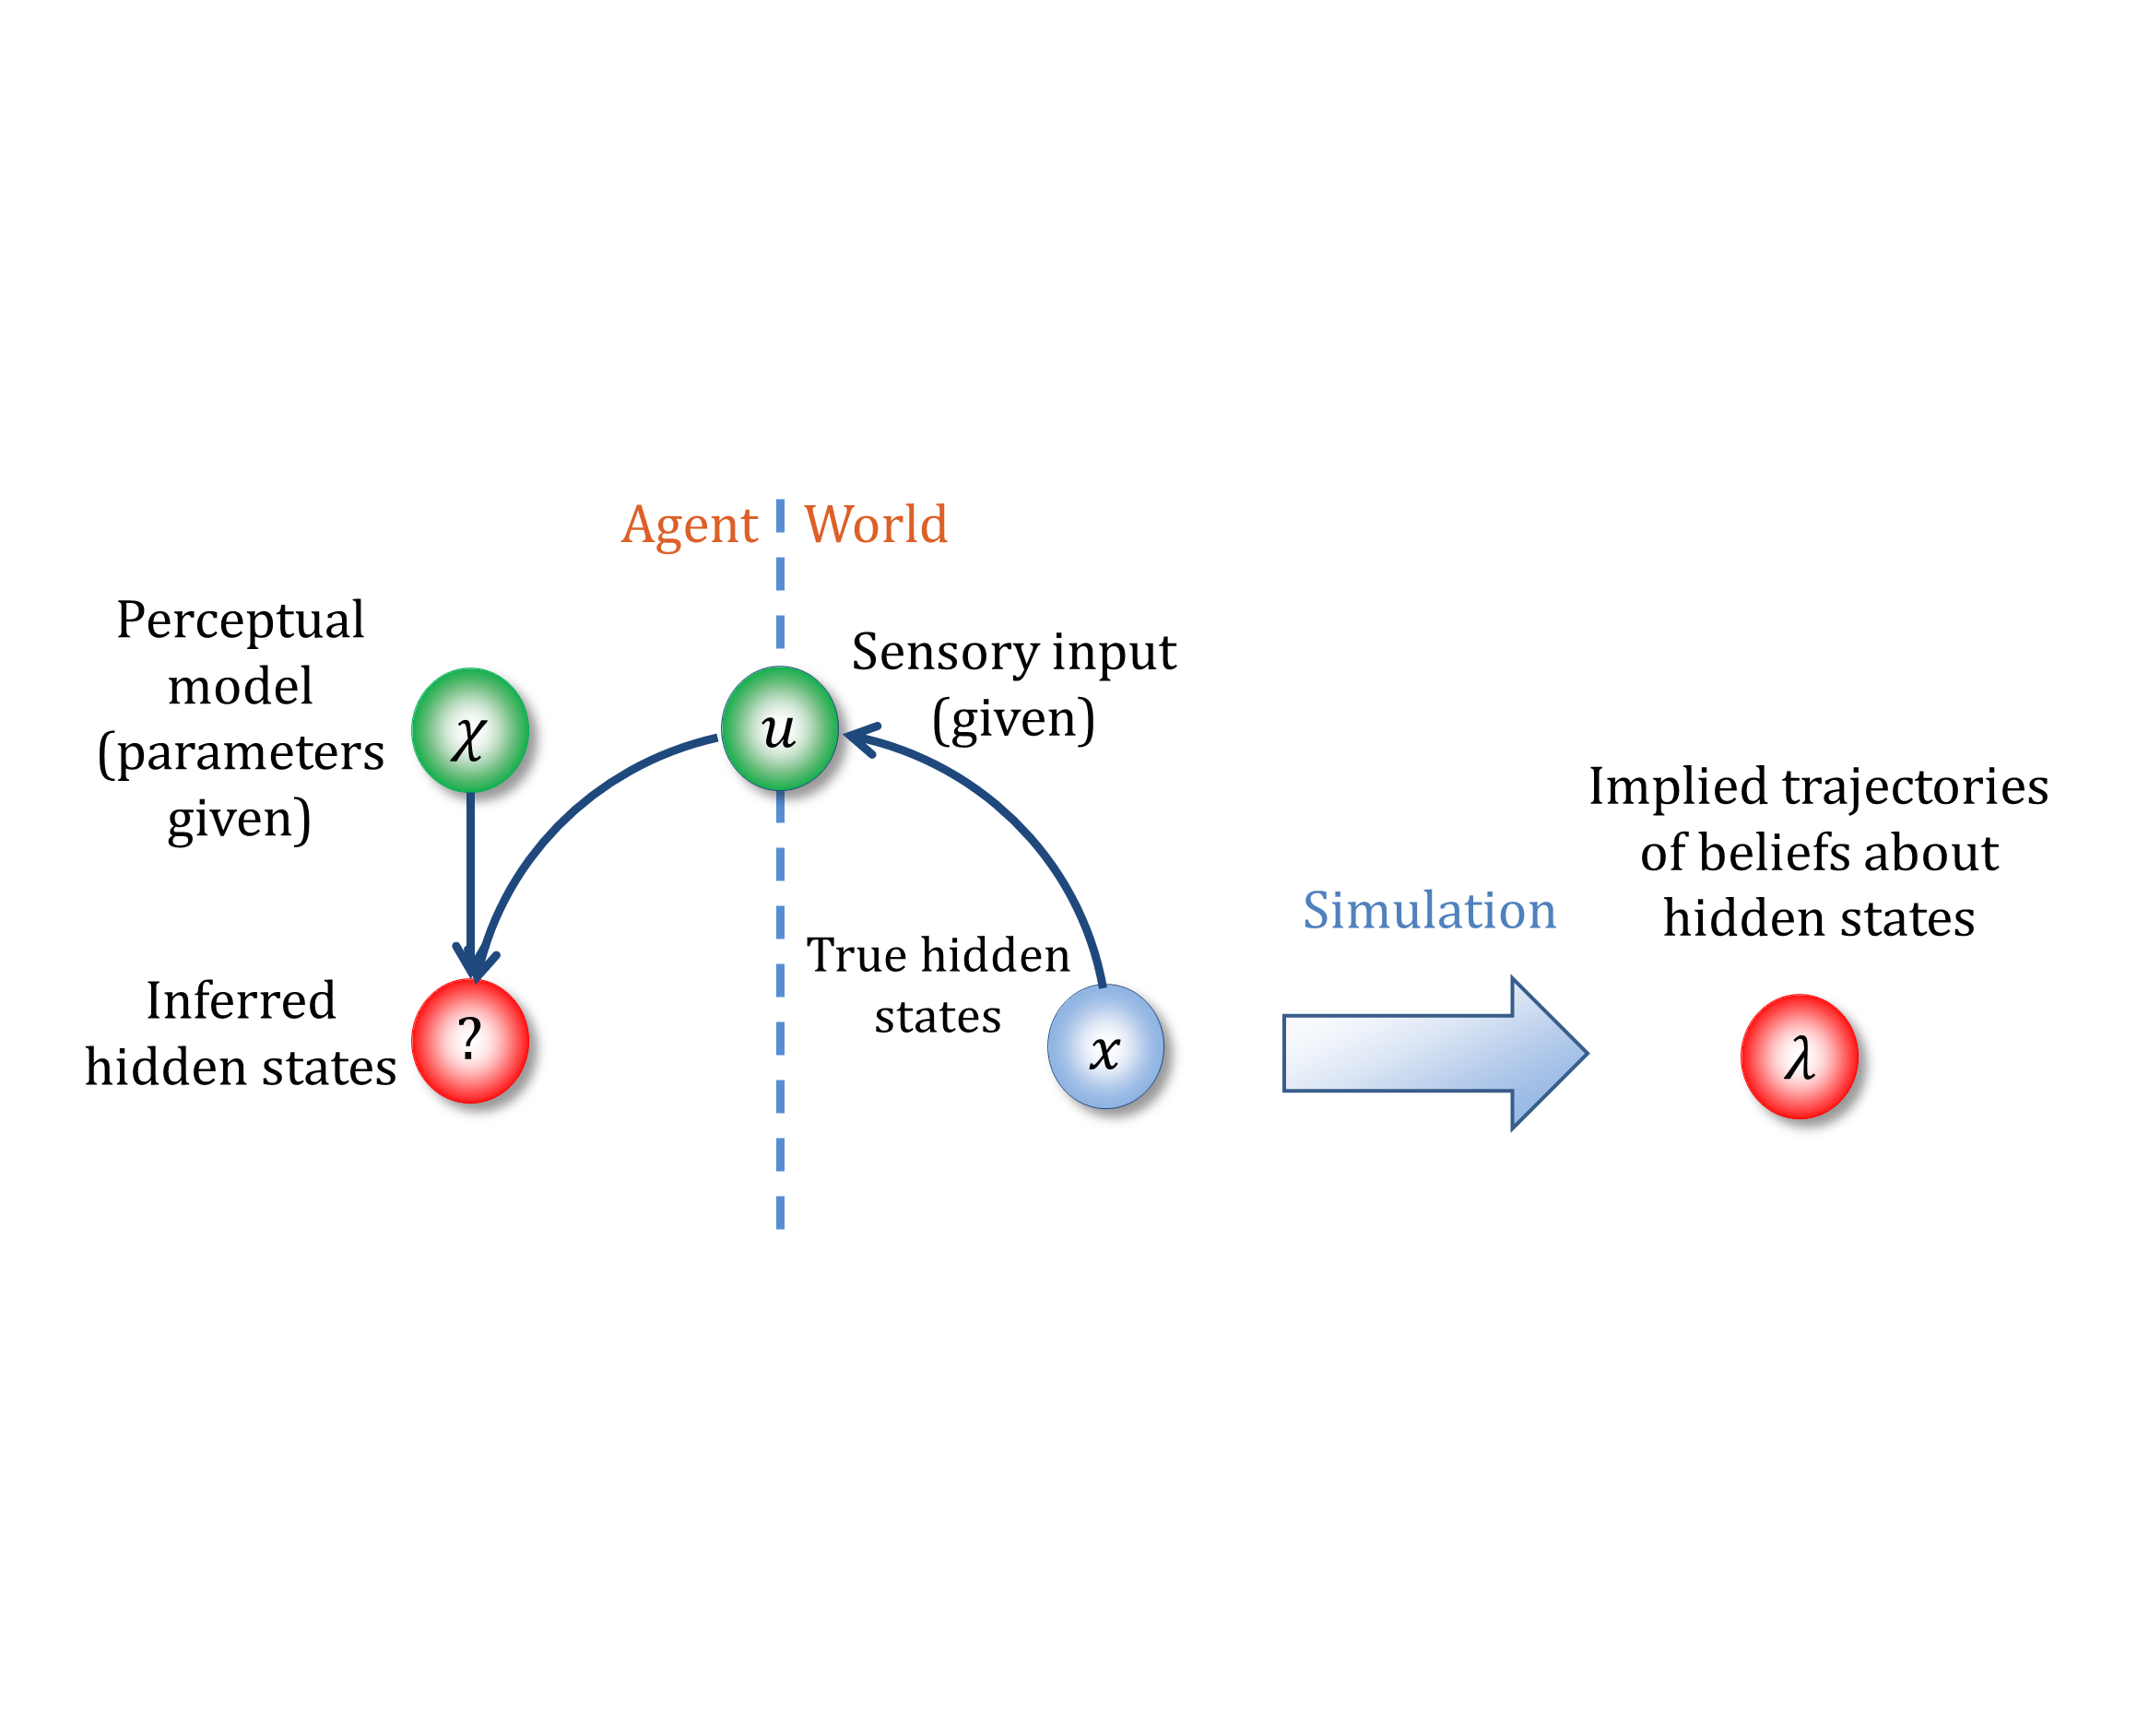
\includegraphics[width=14cm]{Graphics/Slide4}

\vspace{1ex}
\parbox{14cm}{\caption{\label{Slide4}
\textbf{\upshape Simulation of belief trajectories only.}
The function \texttt{\upshape tapas\_simModel(...)} can be called
without specifying a response model.}}
\end{center}
\end{figure}
 
\section{Installation}
\label{sec:install}

Move the main folder with all its contents to a location of your
choice and add it to your Matlab path.


\section{Documentation and tutorial demo}
\label{sec:doc}

Documentation is contained in this manual and throughout the code. To
find out what a particular file does, consult the comments at the head
of its source code.

A good way to get started with the toolbox is to do the tutorial demo
by opening \texttt{hgf\_demo.mlx} in Matlab. A PDF version is
available in \texttt{hgf\_demo.pdf}. This walks you through the main
ways to use the toolbox.

\section{Main functions}
\label{sec:mainfunc}

Each of the two usages (cf. Section \ref{sec:usage}) has its main function. The function

\begin{verbatim}
    tapas_fitModel(...)
\end{verbatim}

fits models to observed responses, while the function

\begin{verbatim}
    tapas_simModel(...)
\end{verbatim}

simulates the trajectories of perceptual states and responses. These
two main functions will be explained in turn in what follows.

\subsection{tapas\_fitModel(...)}
\label{sec:fitmodel}

\subsubsection{Background}

In order to fit a model, you have to make three choices:

\begin{enumerate}
\item A perceptual model,
\item A response model, and
\item An optimization algorithm.
\end{enumerate}

The perceptual model can for example be a Bayesian generative model of
the states of an agent's environment (like the HGF) or a reinforcement
learning algorithm (like Rescorla-Wagner). It describes the
states or values that probabilistically determine observed responses.

The response model describes how the states or values of the
perceptual model map onto responses. Examples are the softmax decision
rule or the closely related unit-square sigmoid decision model.

The optimization algorithm is used to determine the
maximum-a-posteriori (MAP) estimates of the parameters of both the
perceptual and decision models. Its objective function is the
unnormalized log-posterior of all perceptual and response
parameters, given the data and the perceptual and response
models. This corresponds to the log-joint of data and parameters,
given the models.

Perceptual and response models have to be chosen so that they are
compatible, while the choice of optimization algorithm is
independent.

\subsubsection{Configuration}

Once you have made your choice, go to the relevant configuration files
(e.g., \linebreak\texttt{tapas\_hgf\_binary\_config.m}), read the model- and
algorithm-specific information there, and configure accordingly.

Usage then is:

\begin{verbatim}
    >> est = tapas_fitModel(responses, inputs, <prc_model>,
                                     <obs_model>, <opt_algo>);
\end{verbatim}

where the last three arguments are strings containing the names of the
corresponding configuration files (without the extension \texttt{.m}).

These last three arguments are optional. If they are omitted the
defaults configured in \texttt{tapas\_fitModel.m} are used.

\subsubsection{Using placeholder values}

For inputs that lie on a continuous scale, the configuration files of
some perceptual models accept placeholders that are replaced by values
derived from the inputs at runtime (see the documentation in the
relevant configuration files). This makes it easy to automatically
set, for example, the prior mean of the main quantity of interest the
value of the first input.

\subsubsection{Usage}

\begin{verbatim}
     >> est = tapas_fitModel(responses, inputs);
\end{verbatim}
 
\subsubsection{Input arguments}

\begin{description}
    \item{\texttt{responses}}

      Array of binary responses (column vector(s))

    \item{\texttt{inputs}}

      Array of inputs (column vector(s))

      Code irregular (missed, etc.) responses as \texttt{NaN}. Such
      responses will be ignored. However, the trial as such will not
      be ignored and filtering will take place based on the input.
      
      To ignore a trial, code the input as \texttt{NaN}. In this case, filtering is
      suspended for this trial and all representations (i.e., inferences on
      hidden states) will remain constant.

      Note that an input is often a composite event, for example a
      cue-stimulus contingency. If the agent you are modeling is
      learning such contingencies, inputs have to be coded in
      contingency space (e.g., blue cue $\rightarrow$ reward as well
      as green cue $\rightarrow$ no reward is coded as 1 while blue
      cue $\rightarrow$ no reward as well as green cue $\rightarrow$
      reward is coded as 0). The same applies to responses.
      
      If needed for a specific application, responses and inputs can be
      matrices with further columns. The coding of irregular and ignored
      trials described above then applies to their first column.
\end{description}        

\subsubsection{Output}

\begin{description}
  \item{\texttt{est.u}}

    Input to agent (i.e., the inputs array from the arguments)

  \item{\texttt{est.y}}

    Observed responses (i.e., the responses array from the arguments)

  \item{\texttt{est.irr}}

     Index numbers of irregular trials

   \item{\texttt{est.ign}}

     Index numbers of ignored trials

   \item{\texttt{est.c\_prc}}

     Configuration settings for the chosen perceptual model (see the
     configuration file of the model in question for details)

   \item{\texttt{est.c\_obs}}

     Configuration settings for the chosen observation model (see the
     configuration file of the model in question for details)

   \item{\texttt{est.c\_opt}}

     Configuration settings for the chosen optimization algorithm (see
     the configuration file of the algorithm in question for details)

   \item{\texttt{est.optim}}

     A place where information on the optimization results is stored
     (e.g., measures of model quality like LME, AIC, BIC, and
     posterior parameter correlation)

   \item{\texttt{est.p\_prc}}

     Maximum-a-posteriori estimates of perceptual parameters (see the
     configuration file of your perceptual model for details)

   \item{\texttt{est.p\_obs}}

     Maximum-a-posteriori estimates of observation parameters (see the
     configuration file of your observation model for details)

   \item{\texttt{est.traj}}

     Trajectories of the environmental states tracked by the
     perceptual model (see the configuration file of that model for
     details)

\end{description}

\subsubsection{New datasets}

When analyzing a new dataset, take your inputs and use
\texttt{tapas\_bayes\_optimal\_config} (or
\texttt{tapas\_bayes\_optimal\_binary\_config} for binary inputs, or
similar depending on your perceptual model) as your observation
model. This determines the Bayes optimal perceptual parameter values
(i.e., the parameter values that result in the agent being least
surprised overall at the inputs it receives). You can then use the
optimal parameter values as your new prior means.

\subsubsection{Plotting of results}

To plot the trajectories of the inferred perceptual states (as implied
by the estimated parameters), there is a function
\texttt{tapas\_<modelname>\_plotTraj(...)} for each perceptual
model. This takes the structure returned by
\texttt{tapas\_fitModel(...)} as its only argument.

Additionally, the function \texttt{tapas\_fit\_plotCorr(...)} plots
the posterior correlation of the estimated parameters. It takes the
structure returned by \texttt{tapas\_fitModel(...)} as its only
argument. Note that this function only works if the optimization
algorithm makes the posterior correlation available in
\texttt{est.optim.Corr}.

Diagnostics of the residuals of the response model can be plotted
using \linebreak\texttt{tapas\_fit\_plotResidualDiagnostics(...)}.

Detailed examples of workflows including diagnostics are included in
the tutorial demo contained the Matlab LiveScript
\texttt{hgf\_demo.mlx}.

\subsubsection{Usage example}

\begin{verbatim}
     >> est = tapas_fitModel(responses, inputs);
     >> tapas_hgf_binary_plotTraj(est)
     >> tapas_fit_plotCorr(est)
\end{verbatim}

\subsubsection{Bayesian parameter averaging}

It is often useful to average parameters from several estimations, for
instance to compare groups of subjects. This can be achieved by using
the function
\linebreak\texttt{tapas\_bayesian\_parameter\_average(...)} which
takes into account the covariance \linebreak structure between the
parameters and weights individual estimates according to their
precision.

Bayesian parameter averaging only works for estimates that are based
on the same priors and should only be used with care for estimates
based on different inputs.

\subsubsection{Model comparison}

For each model estimation, the toolbox calculates three measures
of model goodness that can be used for model comparison. The first of
these is the log-model evidence (LME), calculated as the negative
variational free energy under the Laplace assumption. In addition to
the LME, AIC and BIC are calculated, which in turn are approximations
to the negative variational free energy. This makes the LME the
measure of choice for model comparison, while AIC and BIC are only
provided because some audiences are more familiar with them.

LMEs can be used to calculate Bayes factors by exponentiating the
difference in LME between two models applied to the same dataset.  For
example, an LME difference of 3 implies a Bayes factor of about 20.

For a fixed-effects analysis with several datasets (e.g., from
different subjects), add up the LMEs for the different datasets and
compare the LME sums.

For a random-effects analysis, use the function \texttt{spm\_BMS(...)}
from the SPM software package (http://www.fil.ion.ucl.ac.uk/spm/) and
see \citet{stephan_bayesian_2009} for the theoretical
background.


\subsection{tapas\_simModel(...)}
\label{sec:simmodel}

\subsubsection{Background}

In order to simulate perceptual states (and, optionally, responses) in
this framework, one has to choose a perceptual model (and, optionally,
an observation model to simulate responses).

The perceptual model can for example be a Bayesian generative model of
the states of an agent's environment (like the HGF) or a reinforcement
learning algorithm (like Rescorla-Wagner). It describes the
states or values that probabilistically determine observed responses.

The observation model describes how the states or values of the
perceptual model map onto responses. Examples are the softmax decision
rule or the closely related unit-square sigmoid decision model.

\subsubsection{Usage}

\begin{verbatim}
     >> sim = tapas_simModel(inputs, prc_model, prc_pvec,
                                       obs_model, obs_pvec);
\end{verbatim}

\subsubsection{Input arguments} 

\begin{description}
  \item{\texttt{inputs}}

    Array of inputs (column vector(s))

    To ignore the input of a trial, code the input as NaN. In this
    case, filtering is suspended for this trial and all
    representations (i.e., inferences on hidden states) will remain
    constant.

    Note that an input is often a composite event, for example a
    cue-stimulus contingency. If the agent you are modeling is learning
    such contingencies, inputs have to be coded in contingency space
    (e.g., blue cue $\rightarrow$ reward as well as green cue
    $\rightarrow$ no reward is coded as 1 while blue cue $\rightarrow$
    no reward as well as green cue $\rightarrow$ reward is coded as
    0). The same applies to responses.

    If needed for a specific application, inputs can be a matrix with
    further columns. The coding of ignored trials described above then
    applies to its first column.

  \item{\texttt{prc\_model}}

    The perceptual model (e.g., \texttt{tapas\_hgf} or \texttt{tapas\_hgf\_binary})

  \item{\texttt{prc\_pvec}}

    Row vector of perceptual model parameter values (see the
    corresponding model's configuration file).

  \item{\texttt{obs\_model}}

    The observation model (e.g., \texttt{tapas\_gaussian\_obs} or \texttt{tapas\_softmax\_binary})

  \item{\texttt{obs\_pvec}}

    Row vector of observation model parameter values (see the
    corresponding model's configuration file).

\end{description}

The last two input arguments are optional. If they are missing, no
responses will be simulated.

To learn more about the various perceptual and observation models,
refer to the comments in their configuration files (e.g., for
\texttt{tapas\_hgf\_binary} to
\linebreak\texttt{tapas\_hgf\_binary\_config.m}).

\subsubsection{Output}

\begin{description}
  \item{\texttt{sim.u}}

    Input to agent (i.e., the inputs array from the arguments)

\item{\texttt{sim.ign}}

  Index numbers of ignored trials

\item{\texttt{sim.c\_sim}}

  Information on the models used in the simulation

\item{\texttt{sim.p\_prc}}

  The perceptual parameters as given in \texttt{pvec\_prc} in the
  configuration file of the perceptual model.

\item{\texttt{sim.p\_obs}}

  The observation parameters as given in \texttt{pvec\_obs} in the
  configuration file of the observation model.

\item{\texttt{sim.traj}}

  Trajectories of the environmental states tracked by the perceptual
  model (see the configuration file of that model for details)

\item{\texttt{sim.y}}

  Simulated responses
\end{description}

\subsubsection{Plotting of results}

To plot the trajectories of the perceptual states implied by the
chosen parameter values, there is a function
\texttt{tapas\_<modelname>\_plotTraj(...)}  for each perceptual
model. This takes the structure returned by
\texttt{tapas\_simModel(...)} as its only argument.

\subsubsection{Usage example}

\begin{verbatim}
     >> sim = tapas_simModel(u, 'tapas_hgf_binary',
                  [NaN 0 1 NaN 1 1 NaN 0 0 NaN 1 NaN -2.5 -6],
                  'tapas_unitsq_sgm', 5);
     >> tapas_hgf_binary_plotTraj(sim)
\end{verbatim}

\section{Adding models}
\label{sec:addmod}

Owing to its modular structure, the toolbox allows you to add
perceptual and observation models of your choice. This requires the
following files containing the corresponding functions that
\texttt{tapas\_fitModel(...)} and \texttt{tapas\_simModel(...)}  will
expect to find (replace \texttt{<modelname>} by the name of your
model):

\begin{description}
\item{\texttt{tapas\_<modelname>.m}}

  Contains the model machinery

\item{\texttt{tapas\_<modelname>\_config.m}}

  Contains the configuration settings (only for
  \texttt{tapas\_fitModel(...)})

\item{\texttt{tapas\_<modelname>\_transp.m}}

    Transforms parameters from the space they are estimated in to
    their native space (only for \texttt{tapas\_fitModel(...)} and
    \texttt{tapas\_bayesian\_parameter\_average(...)})

\item{\texttt{tapas\_<modelname>\_namep.m}}

  Returns a structure of named parameters (only for
  \texttt{tapas\_simModel(...)})
\end{description}

Additionally, for observation models, \texttt{tapas\_simModel(...)}
expects to find a function that performs the simulation of responses:

\begin{verbatim}
     tapas_<modelname>_sim.m
\end{verbatim}

For details, look at the corresponding files of an existing model
(e.g., \texttt{tapas\_hgf\_binary.m,} etc.) and use them as templates.


\section{Adding optimization algorithms}
\label{sec:addoptalgo}

To add a new optimization algorithm, provide the following functions
that \linebreak\texttt{tapas\_fitModel(...)} will expect to find (replace
\texttt{<algo>} by the name of your algorithm):

\begin{description}
\item{\texttt{tapas\_<algo>}}

Contains the machinery of the algorithm

\item{\texttt{tapas\_<algo>\_config}}

Contains the configuration settings
\end{description}

For details, see the corresponding files of an existing algorithm
(e.g., \linebreak\texttt{tapas\_quasinewton\_optim.m}) and use them as
templates.

\section{Selection of published studies using the toolbox}
\label{sec:pubstud}

In addition to papers cited throughout, the references at
the end of this manual contain a selection of published studies where
the HGF Toolbox was used.

\nocite{*}
\bibliographystyle{psyinst-en}
\bibliography{hgfToolBox}

\end{document}
%  LocalWords:  addmod citet mathys renewcommand baselinestretch hgf
%  LocalWords:  includegraphics vspace textbf upshape daunizeau prc
%  LocalWords:  texttt mainfunc fitmodel subsubsection linebreak pvec
%  LocalWords:  rightarrow est.irr est.ign est.optim est.traj stephan
%  LocalWords:  plotTraj simmodel sim.ign sim.traj transp.m optim.m
%  LocalWords:  addoptalgo quasinewton pubstud nocite
